% TO BE INSERTED INTO ACRONYMS SECTION:

% SSG - symbolic state graph
% CFG - control flow graph
% BB - Basic Block

% tala en highlevel description of implementation, liknande revgen paper section 4.
% https://dslab.epfl.ch/pubs/revgen.pdf

\begin{figure}
    \centering
    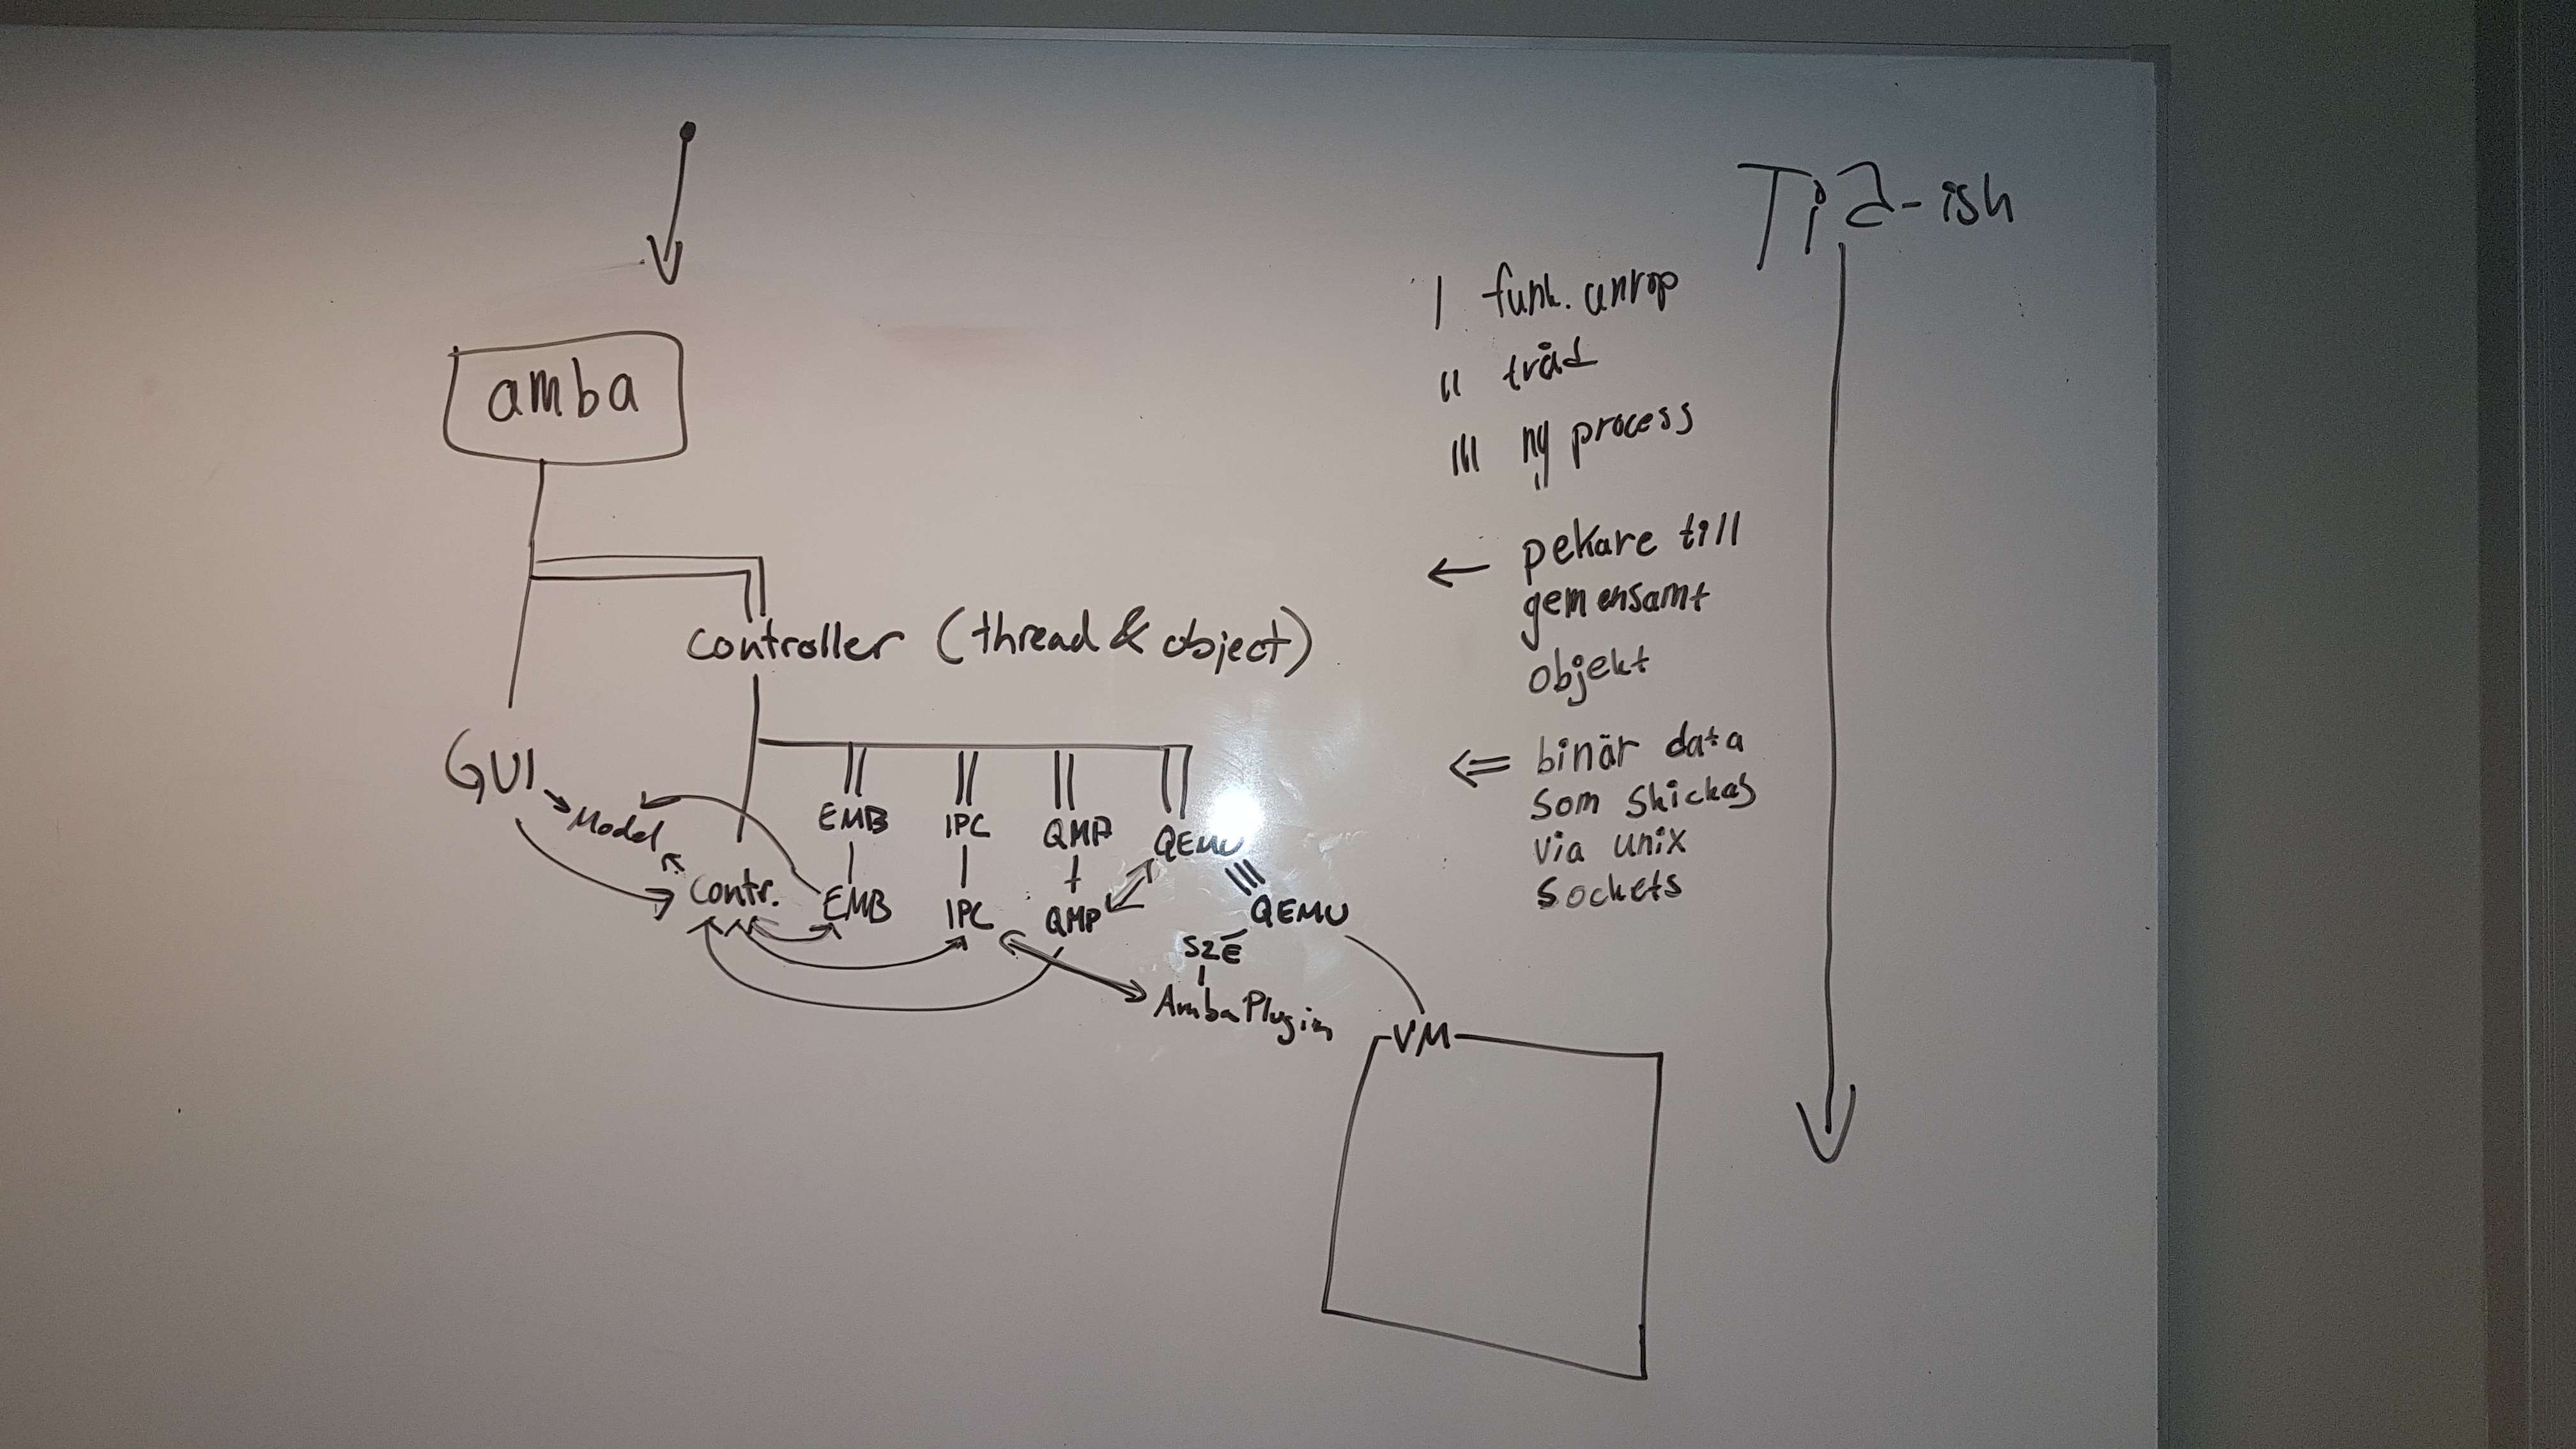
\includegraphics[width=\textwidth]{figures/arkitektur.jpg}
    \caption{Placeholder: Systemöversikt över AMBA}\label{fig:arkitektur}
\end{figure}

%

AMBA ska betraktas som ett system bestående av ett flertalet subsystem
som kommunicerar med varandra med delade objekt eller unix socklar.
Systemet tar som indata en configurationsfil som bland annat
specificerar sökvägen till binären som ska analyseras samt
inställningar till S2E.  Utdatan är en interaktiv graf baserad på
symboliska uttryck som baseras på binärens maskinkod.  Grafen ger en
visualisering över vilka möjliga vägar som exekveringen kan ta när
binären körs på en maskin.  En översikt av systemets arkitektur finns
i figur~\ref{fig:arkitektur}.  Med hjälp av inställningarna från
konfigurationsfilen startas sedan QEMU och \stoe{} med vårt \stoe{} plugin
AmbaPlugin.  Ett operativsystem och binären laddas in och börjar
exekveras. \stoe{} anropar callbackfunktioner definierade i
AmbaPlugin, vilka är tillagda i utvalda \stoe{} hooks, som sedan
uppdaterar vyn i vislualiseringen.

\section{Amba}

% Outline
% 1. Läser in en Recipe fil. (insällningar till s2e)
% (optional) 2. Startar GUI
% 3. Spawnar controller thread (gui gör det om man kör med GUI, annars amba direkt)
% 4. Controller spawnar QEMU (S2E); QMP listener (kommunikation mellan
%     controller och QEMU); IPC mekanism mellan libamba och controller; och
%     Embedder som layoutar en 2D graph för visualisering givet en CFG.

\section{S2E}
S2E använder sig av en modifierad QEMU instans för exekvering av olika
binärer och har en modulär arkitektur bestående av plugin som
möjliggör analys av binärer. Plugin har möjlighet att följa S2E:s
exekvering och undersöka egenskaper för att spåra och forma
analyser~\cite{Chipounov12}.

Konceptuellt består ett S2E plugin av ett tillstånd och en
initieringsfuktion. Tillståndet ärvs från ett kärn-plugin som
innehåller information om bl.a.\ programtillstånd, symbolisk
exekveringstillstånd och information om andra plugin. Tillståndet kan
utökas för att samla information, kontrollera egenskaper och utföra
binäranalys. Initieringsfunktionen består av tillståndsinitiering och
registrering av callbacks till olika hooks som tillgängligörs av
antingen S2E:s kärn-plugin eller andra plugin. Dessa callbacks anropas
under exekvering när motsvarande villkor för en hook uppfylls.

AmbaPlugin är ett S2E plugin som har utvecklats för att samla
information under exekvering av en binär ämnat för att visualisera
exekveringen i AMBA.\@

\section{AmbaPlugin}
AmbaPlugin registrerar callbacks för ett antal hooks bland vilka
\texttt{onStateFork} och \texttt{onBlockStart}.
När dessa hooks aktiveras samlas information om S2E:s state id,
generation för ett block i fallet av självmodifierande kod, uttrycket
för villkoret för att programexekveringen ska nå denna state och ett
id som utdelas till olika states. Utifrån detta framställs
kantinformation för CFG och Symbolisk state graf som kontinuerligt
skickas över IPC till GUI processen. Även annan information om varje
nod i de olika graferna samlas och skickas över IPC till GUI
processen. Denna iterativa informationsuppdateringen är tänkt att
kommunicera framsteg till användaren eftersom exekveringen kan ta lång
tid beroende på den binär som analyseras.

% \section{Nix-miljö för S2E utveckling}
% S2E är ett komplicerat system och består av bland annat QEMU och
% behöver mycket konfiguration för att sätta % upp en miljö för
% symbolisk exekvering. Verktyget \textit{s2e-env} har tidigare
% utvecklats för att underlätta många steg som skapandet av
% gäst-VM-avbild~\cite{s2e_website_s2eenv}. \textit{s2e-env} antar
% däremot \textit{Ubuntu 18.04 LTS 64-bit OS} som värd för att kunna
% hämta rätt beroenden~\cite{s2eenv_github}. Detta % har varit en
% svåröverkomlig krav för utvecklandet av AMBA och därför har en
% nix-miljö framställts för att hantera och bygga alla beroenden som
% krävs för att bygga och köra S2E med QEMU.

% Nix-miljön har framställts för utveckling av AMBA och är inte lämplig
% för upstreaming till \textit{s2e-env} i nuvarande form men kan vara
% möjligt efter utökningar och modifieringar.

\section{GUI}
AMBA-processen använder immediate-mode-gui-biblioteket egui~\cite{egui}
för att rita sitt gränssnitt. Detta innebär att hela fönstret ritas om
varje bildruta. Processen samlar kantinformation som AmbaPlugin
skickar och bygger de tre graferna nämnda tidigare.

\section{[WIP] Grafkoden (rename)}
I grunden består grafen av en avbildning (jmf map) av id:n till noder,
där en nod är tre mängder av id:n som representerar kanter in, kanter
ut och, i den komprimerade grafens fall, vilka noder som slagits
samman för att bli den här noden, sorterad efter ordningen de har i
den underliggande linjegrafen.

% This can't be a figure because latex will then move it too far away
% from the relevant text
% \begin{figure}
% Rust isn't supported, Swift is close enough syntactically
\begin{lstlisting}[label={list:third}, language=Swift]
// Language question: Translate field names to Swedish?
// Specify Set and Map? List -> Vec?
struct Node {
    from:  Set<Id>,
    to:    Set<Id>,
    of:    List<Id>,
}

struct Graph {
    nodes: Map<Id, Node>
}
\end{lstlisting}
% \caption{Typsignaturer i pseudokod}
% \end{figure}

Grafen byggs av en wrappertyp som konverterar från strukter av
metadata till sekventiella id:n. Id:na är sekventiella för att
metadatan ska kunna förvaras i en lista bredvid och använda index som
id. Grafen stödjer byggandet av både råa och komprimerade grafer. När
en kant läggs till i grafen registreras varandras id:n i nodernas
from- och to- set. Om det är en komprimerad graf hittas noderna som
innehåller id:na som ska samman kopplas och bryter dem i två noder var
efter/före id:t i fråga och kopplar dem samman efter det. När kanten
är tillagd kollas det om den är en del av en linjegraf och slår sedan
samman noderna om så är fallet.

\subsection{Nodgruppering}
Noderna i de första två graferna färgas efter starkt anslutna
komponenter (jmf strongly connected components). En starkt ansluten
komponent i en riktad graf är den subgrafen där alla noder kan nå alla
andra noder i subgrafen. Detta beräknas via Tarjan's
Strongly Connected Components Algorithm.~\cite{tarjan}

Noderna kan också färgas efter funktion enligt debuginformation i
associerad DWARF-data.

% s2e_website_s2eenv  url: https://s2e.systems/docs/s2e-env.html
